\documentclass{article}
\usepackage{Sweave}
\usepackage{tabularx}
\usepackage{geometry}
\geometry{margin=.5in}
\usepackage{enumerate}
\usepackage{subfig}
\usepackage[demo]{graphicx}
\makeatletter
\setlength{\@fptop}{0pt}
\makeatother
\begin{document}
\Sconcordance{concordance:figures_page.tex:figures_page.Rnw:%
1 57 1}

%updated May 16 2016
\begin{figure}[!tbp]
  \centering
  \fbox{\subfloat[Physioloical Hysteranthy: Average floral and foliar budburst]{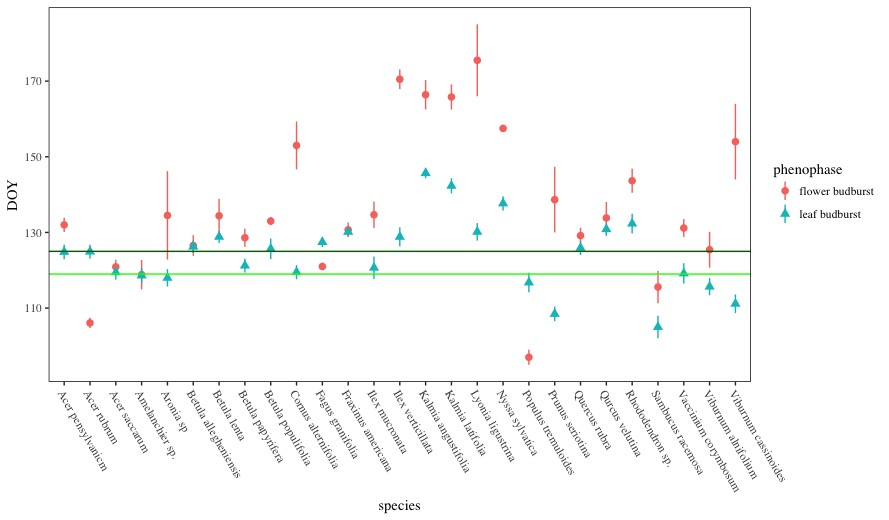
\includegraphics[width=0.5\textwidth]{HF_phys.jpeg}\label{fig:f1}}
  \hfill
  \subfloat[Functional Hysteranthy: Average first flowering and leaves expansion to 75 percent]{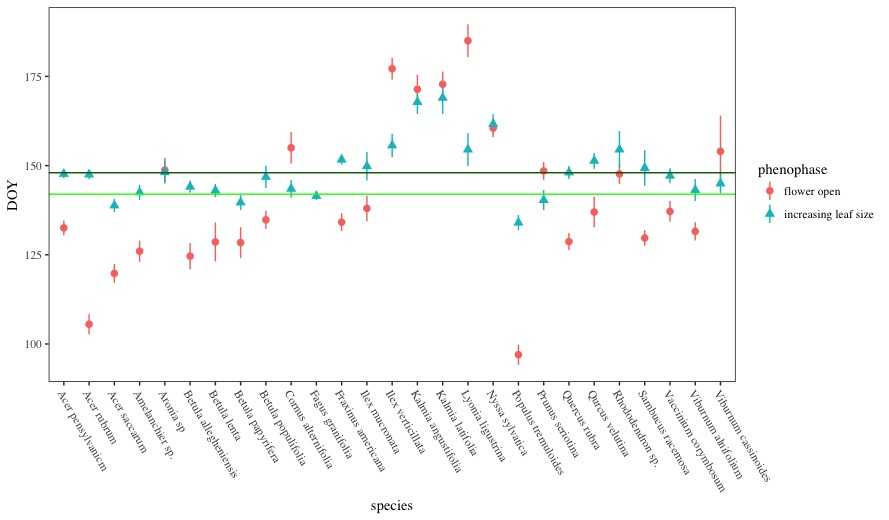
\includegraphics[width=0.5\textwidth]{HF_funct.jpeg}\label{fig:f2}}}
  \caption{Average Floral and Leaf Phenology at Harvard Forest 1990-2014. As seen through comparision, species classifications of hysteranthy vary greatly depending on whether physiologicial or functional definitions are used.}
\end{figure}

\begin{figure}[!tbp]
  \centering
 \fbox{ \subfloat[Acer rubrum]{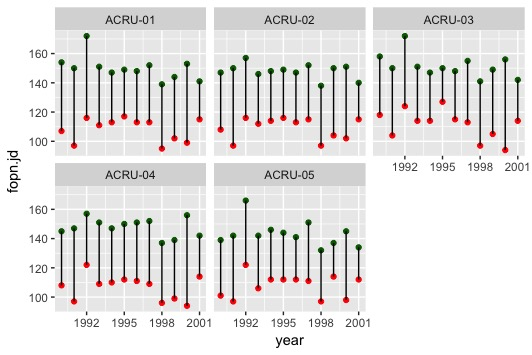
\includegraphics[width=0.33\textwidth]{ACRU.jpeg}\label{fig:f3}}
  \hfill
  \subfloat[Quercus rubra]{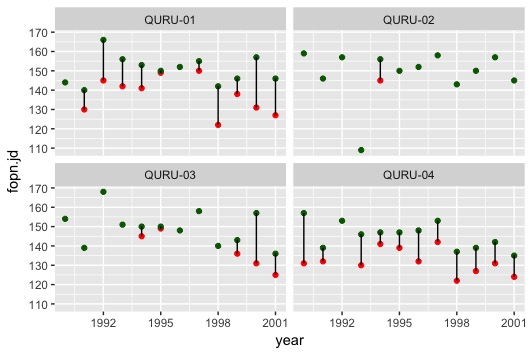
\includegraphics[width=0.33\textwidth]{QURU.jpeg}\label{fig:f4}}
  \subfloat[Betula populifolia]{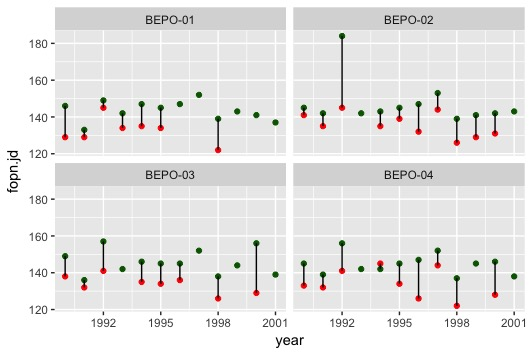
\includegraphics[width=0.33\textwidth]{BEPO.jpeg}\label{fig:f5}}}
  \caption{Annual variation in degree of hysteranthy for individals in Harvard forest 1900-2001.}
\end{figure}

\begin{figure}[!tbp]
  \centering
  \fbox{\subfloat[MTSV]{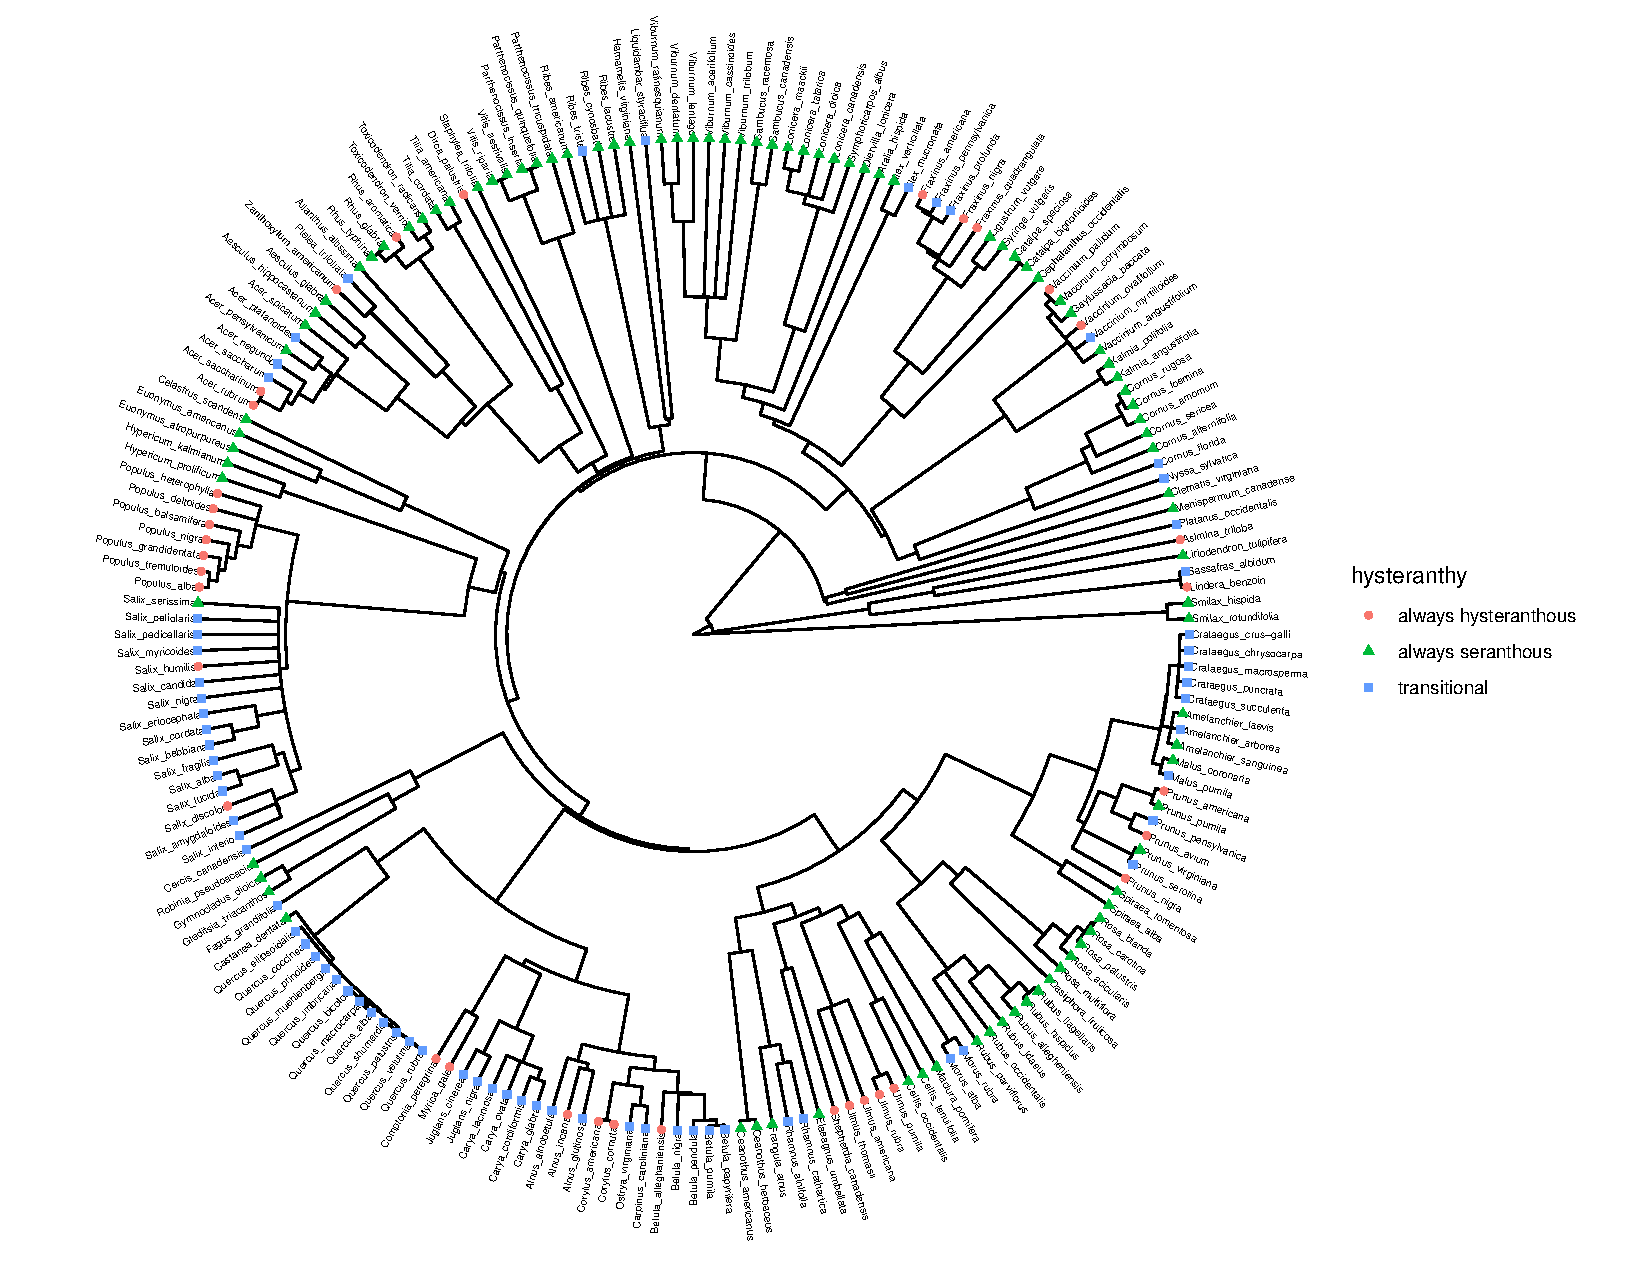
\includegraphics[width=0.5\textwidth]{New_circle_tree.pdf}\label{fig:f1}}
  \hfill
  \subfloat[Silvics]{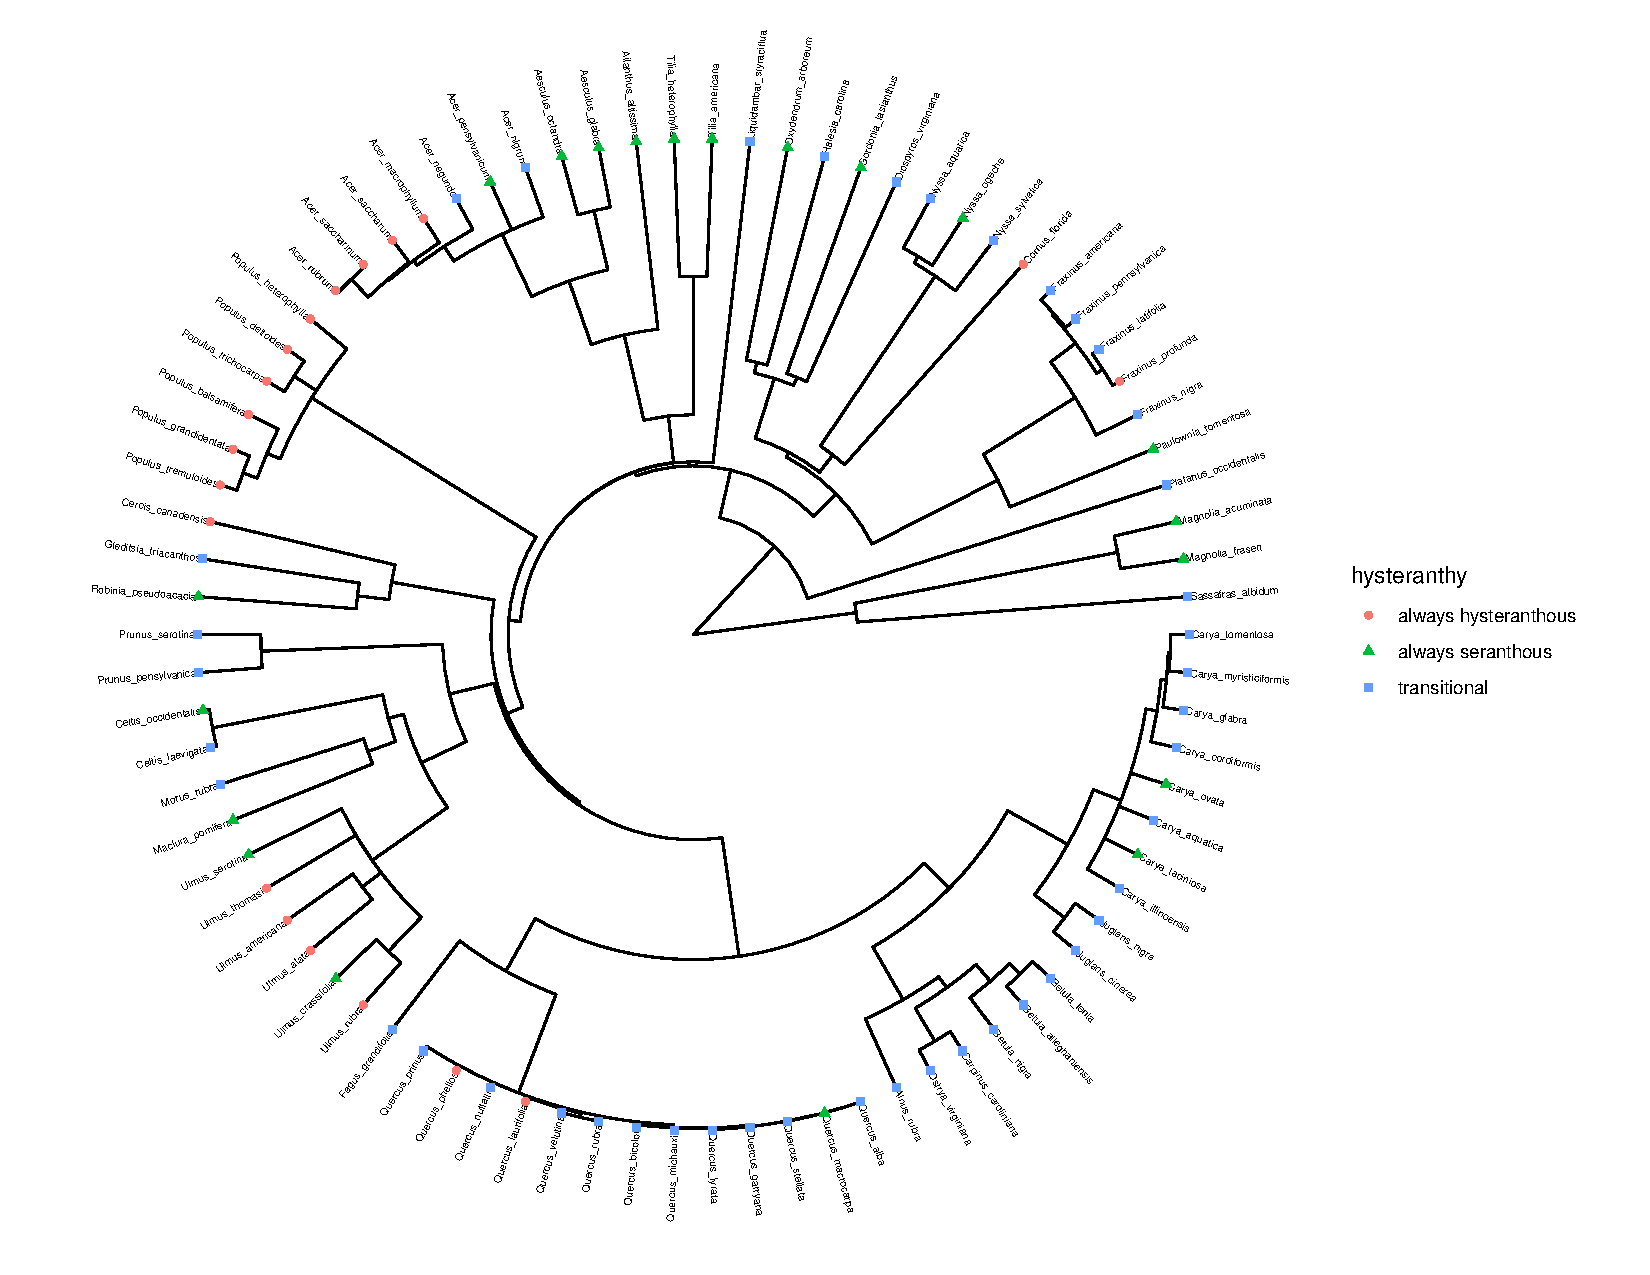
\includegraphics[width=0.5\textwidth]{Circle_tree_silvics.pdf}\label{fig:f2}}}
  \caption{Phylogenies for the two data sets and hysteranthy traits. Blue indicates a reclassification of hysteranthy depeding on which binning metrics used. I should add phyloD values to this figure}
\end{figure}

\begin{figure}[h!]
  \centering
   \fbox{ 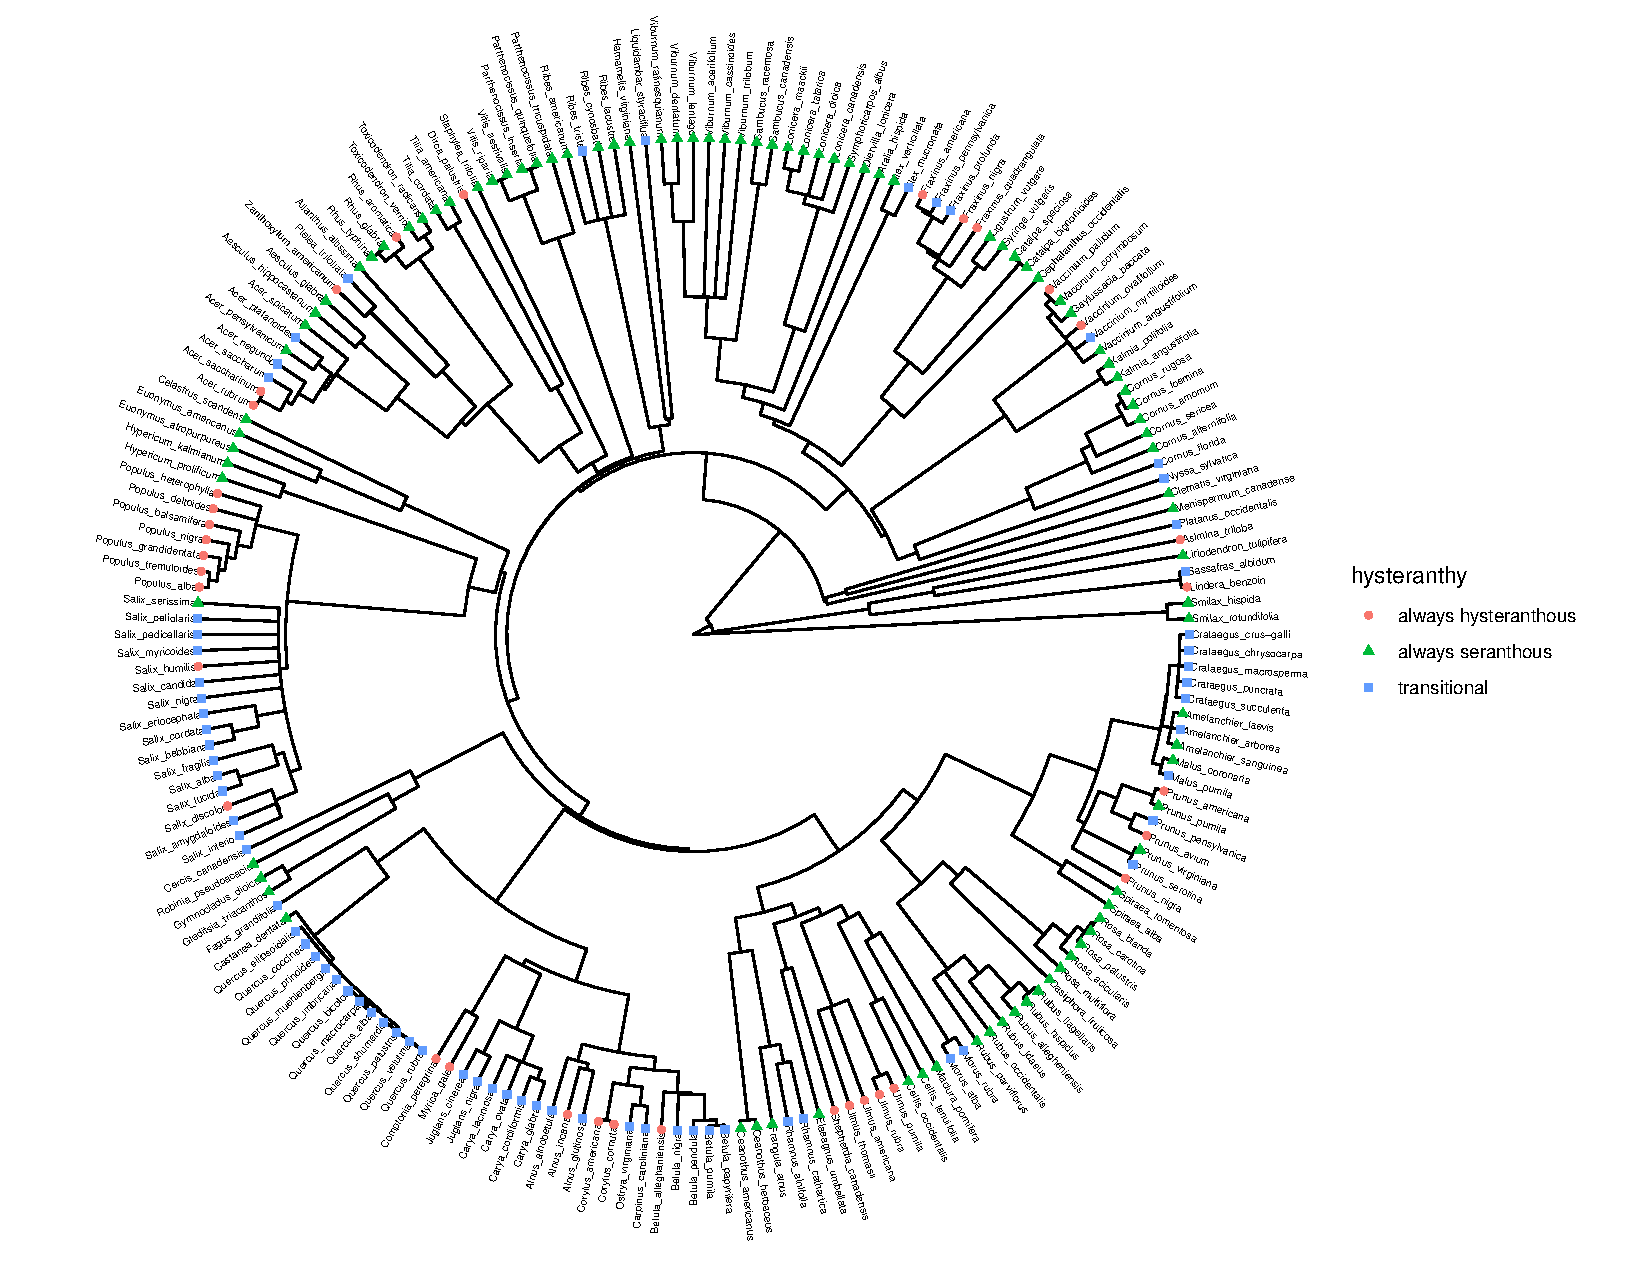
\includegraphics[width=\textwidth]{New_circle_tree.pdf}}
   \caption{Phylogenetic relationships for MTSV data. Blue species get redefined as hysteranthous as when a different definiton is applied. I should add the Phylo D values to this figure}
\end{figure}

\begin{figure}[h!]
  \centering
   \fbox{ 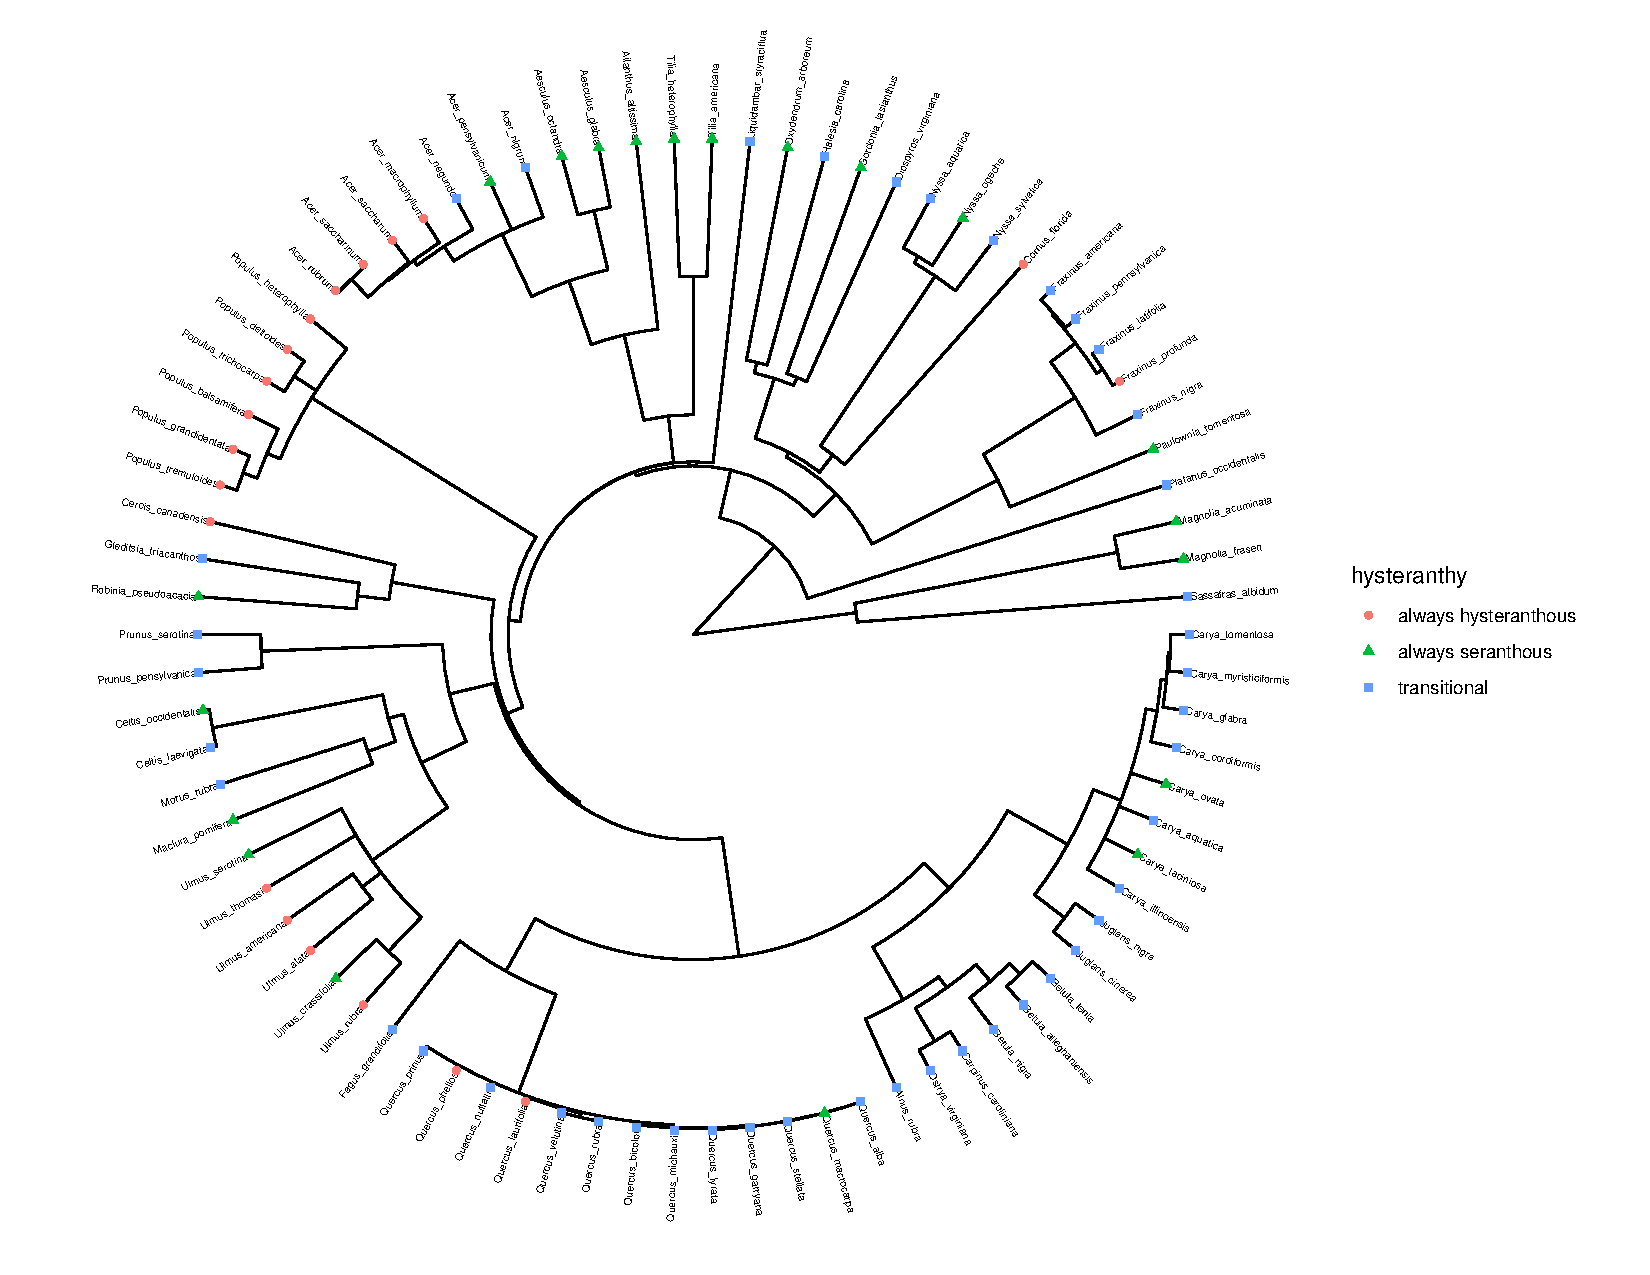
\includegraphics[width=\textwidth]{Circle_tree_silvics.pdf}}
   \caption{Phylogenetic relationships for MTSV data. Blue species get redefined as hysteranthous as when a different definiton is applied}
\end{figure}

\begin{figure}[!tbp]
  \centering
 \fbox{ 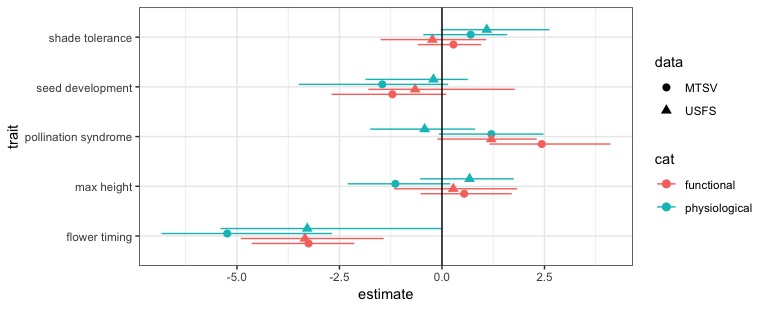
\includegraphics[width=0.95\textwidth]{Data_comparision_plot.jpeg}\label{fig:f6}}
\caption{Golly, we get different outputs.}
\end{figure}




\end{document}
